\section{标准控制台输入输出}
\hfill\ctli{实验时间}{~2014~年~11~月~28~日}

\subsection*{【实验目的】}
\begin{enumerate}[topsep=0pt,partopsep=0pt,itemsep=0pt,parsep=0pt,label={\arabic*、}]
\item 熟悉Dev-Cpp编程环境。
\item 编写简单的输入输出语句。
\item 熟练使用算术运算符。
\item 能够编写简单的判断语句。
\end{enumerate}
\subsection*{【实验环境】}
\MyEnvironment
\subsection*{【实验内容】}
编写C++程序,实现输入两个整数,输出两个整数的加、减、乘、除结果;详细的注释,完整的输出显示。
\subsection*{【详细分析】}
实验内容是简单的对两个输入整数的四则运算,即简单的顺序结构。

在此基础上稍作改动,即输入整数和运算符来自动进行计算,流程如图\ref{aly01}。
\begin{figure}[htp]
\centering
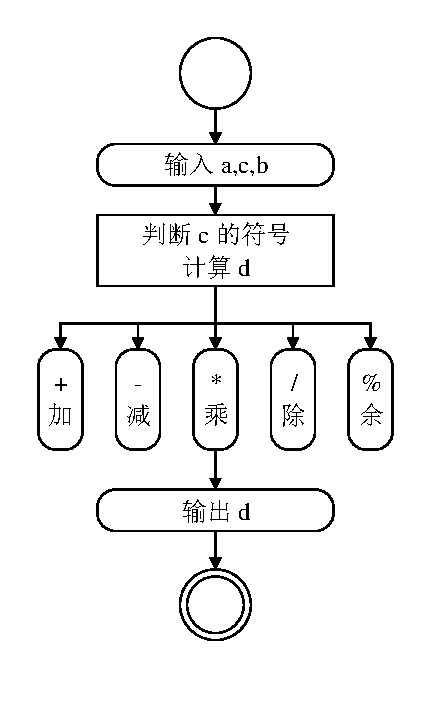
\includegraphics{exp01/exp01.pdf}
\caption{\label{aly01}程序流程图}
\end{figure}
\subsection*{【实验源码】}
{\linespread{1}\lstinputlisting[caption={\tt exp01.cpp}]{exp01/exp01.cpp}}
\subsection*{【实验结果】}
\begin{figure}[htp]
\centering
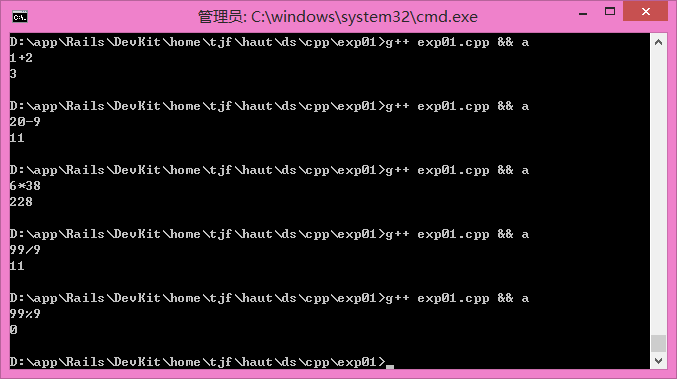
\includegraphics[width=\textwidth]{exp01/exp01.png}
\caption{\label{out01}标准控制台输入输出}
\end{figure}
图\ref{out01}显示了编译、运行、输入、输出的过程。
\subsection*{【实验体会】}
这是一个非常基础的简单程序,目的在于熟悉编程和调试环境。程序本身没有任何难度,加上注释也不过40行。

关于编程环境的配置,我倾向于使用编辑器(如 Vim、Sublime Text)编写源文件,在命令行下编译、运行和调试(使用 gcc/gdb)。当然,Microsoft Visual Studio 作为世界上最好的 IDE ,在编写调试程序中也是非常好用的,所以在有条件的时候也会使用VS。

\clearpage\newpage
